\chapter{Start up}

\begin{enumerate}
	\item Turn on computer and wait until the desktop appears.
	\item Connect the 4 USB-to-Serial adapters in the order of their numbers (On which usb-port which adapter is connected doesn't matter).
	\item Start the stretcher software.
\end{enumerate}

\section{Normal start}
\label{sec:normalstart}
With the start of the stretcher program, a start-up dialog figure \ref{fig:startup} will appear and ask if the mechanical set up has changed.

\begin{figure}[!ht]
	\centering
		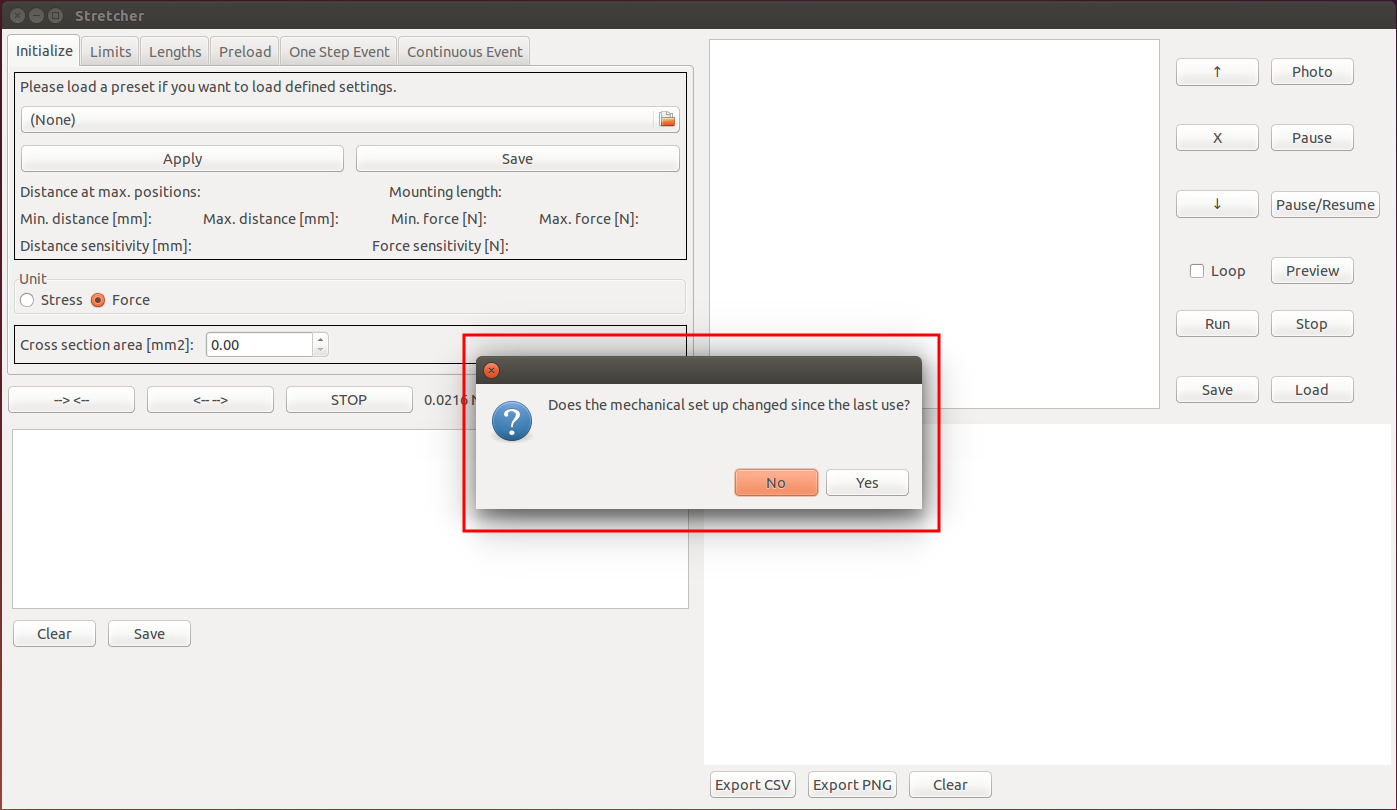
\includegraphics[width=1.0\textwidth]{images/StartUp1}
	\caption{Start-up dialog}
	\label{fig:startup}
\end{figure}

If the mechanical set up has not change, the program will load the parameters from the last usage.
\\
Otherwise, a new dialog will appear, see figure \ref{fig:setdistance} and the user should move the stage to a distance, measure it and insert the measured distance it.

\begin{figure}[!ht]
	\centering
		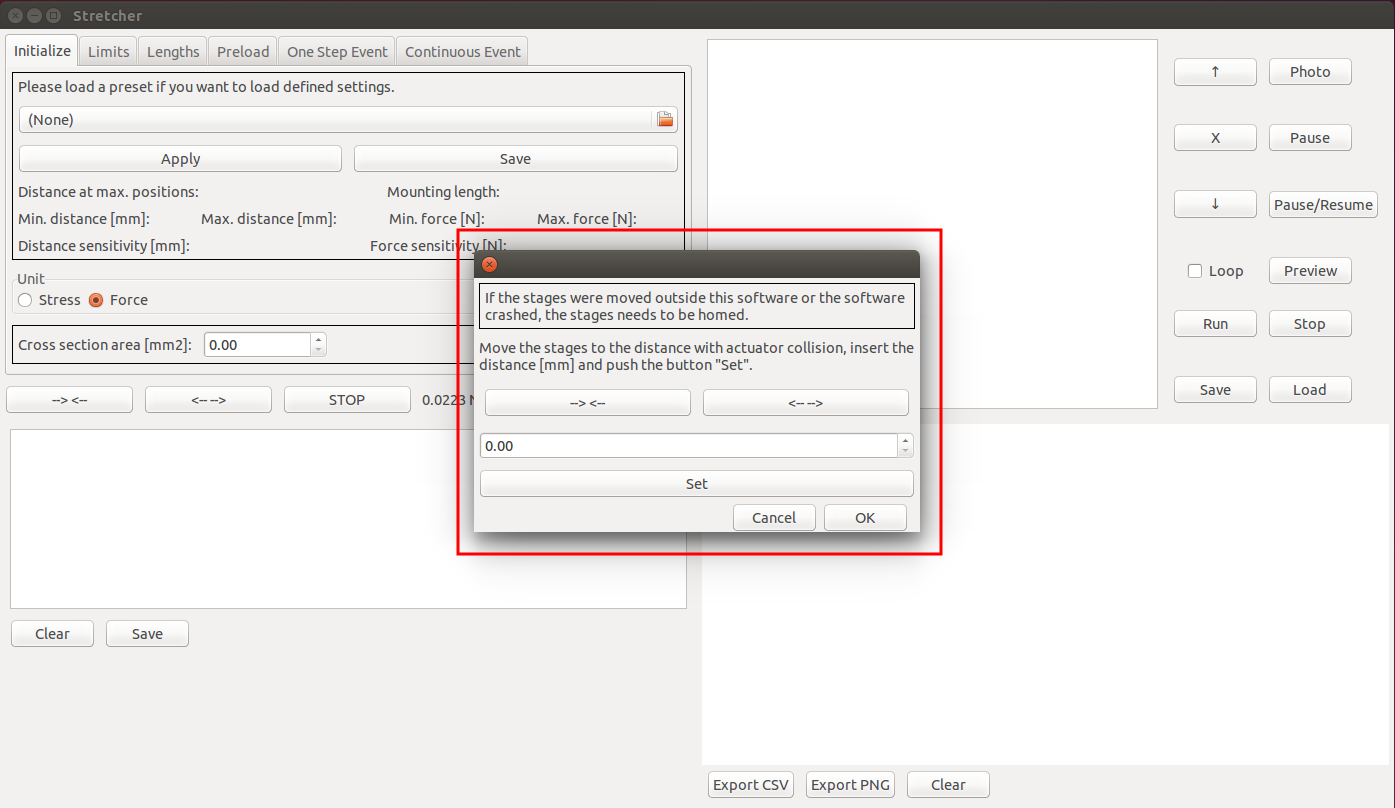
\includegraphics[width=1.0\textwidth]{images/StartUp2}
	\caption{Set distance dialog}
	\label{fig:setdistance}
\end{figure}

In both cases, the current parameters are visible in the tab ``Initialize'', shown in figure \ref{fig:initialize}. In this tab, the user can choose, if the experiments should be force or stress based, by selection the according radio button and in the case of stress, by specifying the cross section area.

\begin{figure}[!ht]
	\centering
		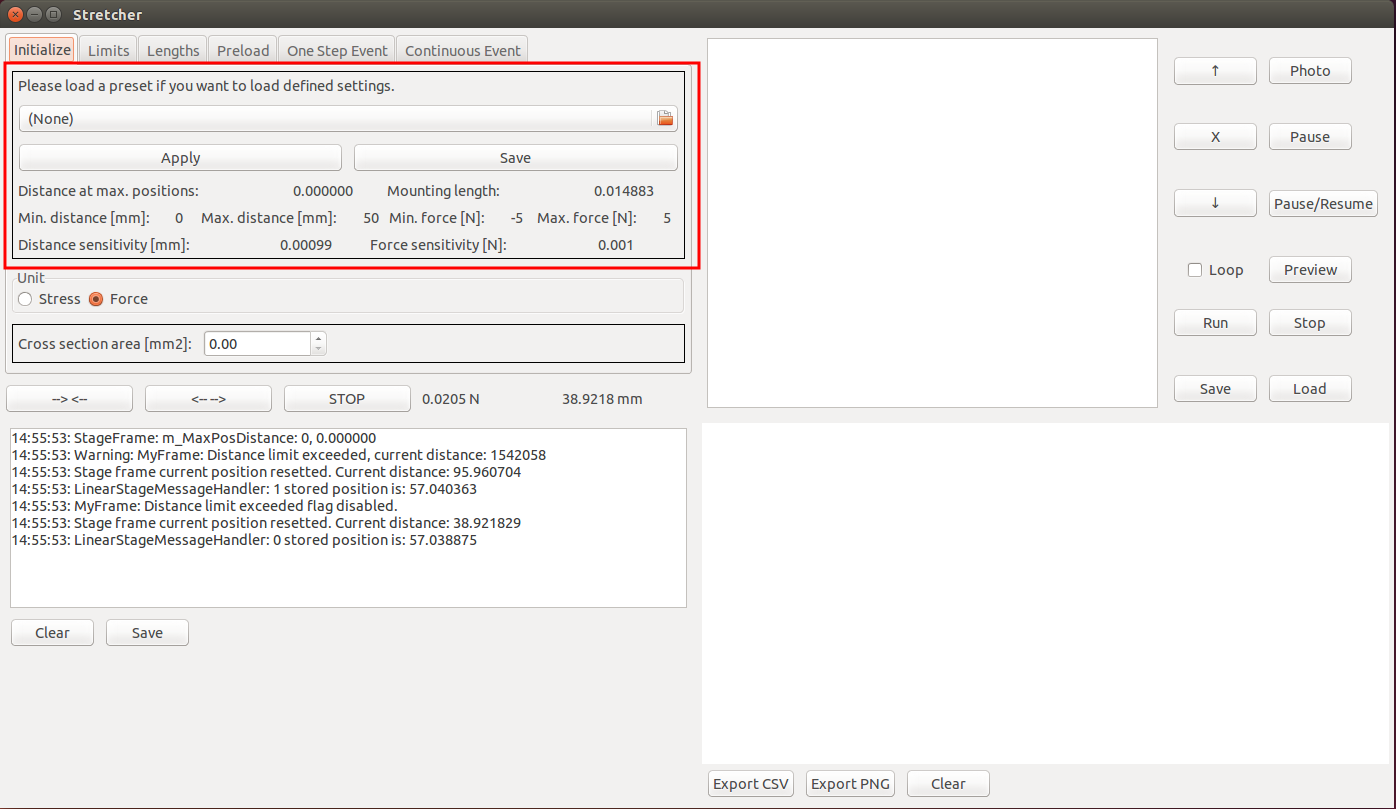
\includegraphics[width=1.0\textwidth]{images/Initialize}
	\caption{Initialize tab}
	\label{fig:initialize}
\end{figure}

In the next step, the user can set/adjust the force/stress and the distance limits. For this the desired values can be chosen in the tab ``Limits'', shown in figure \ref{fig:limits}. The user can either input the desired values or load one of the four limit sets and then apply them by pushing the button ``Set limits''.

\begin{figure}[!ht]
	\centering
		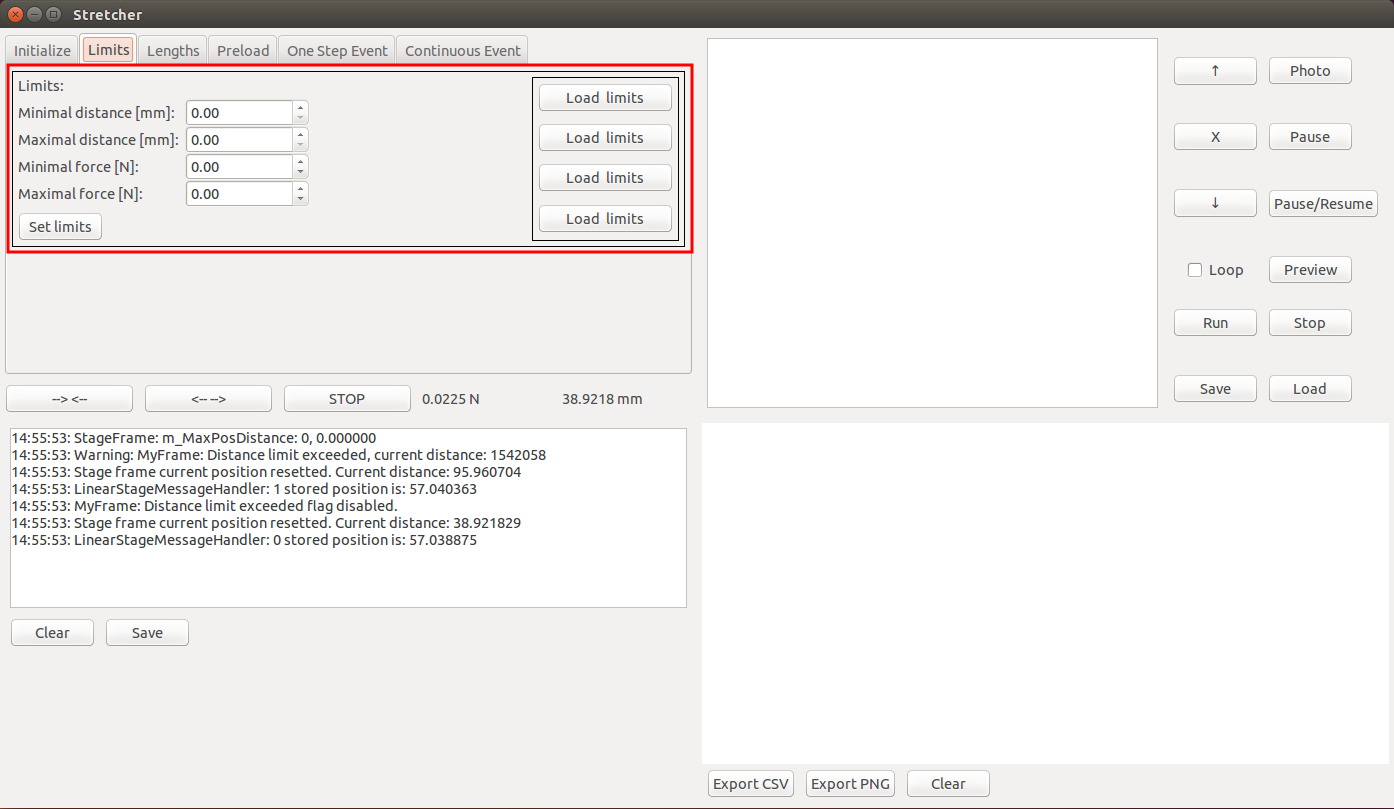
\includegraphics[width=1.0\textwidth]{images/Limits}
	\caption{Limits tab}
	\label{fig:limits}
\end{figure}

After the limits are correct, lengths settings can be adjusted in the tab ``Lengths'', shown in figure \ref{fig:lengths}. In the distance field, the user can insert the desired mounting length and then push the button ``Go to'', which will move the stages to it. It is also possible to use the increase- and decrease button to adjust the distance. When the mounting length is reached, it can be fixed by pushing the button ``Set mounting length''. As next, the the sensitivities for the distance and force or stress values can be defined.


\definecolor{shadecolor}{gray}{0.9}
\begin{narrowframed}
	Note: The sensitivity values are one half of the thresholds used in the experiment to reach a stress, force or distance value. For a better understanding, a value is reached, if the current value \(value_{current}\) is between \(value_{desired} - sensitivity\) and \(value_{desired} + sensitivity\). The sensitivity values have to be chosen according to the used velocity because as higher the velocity as more inaccurate the system becomes.
\end{narrowframed}

\begin{figure}[!ht]
	\centering
		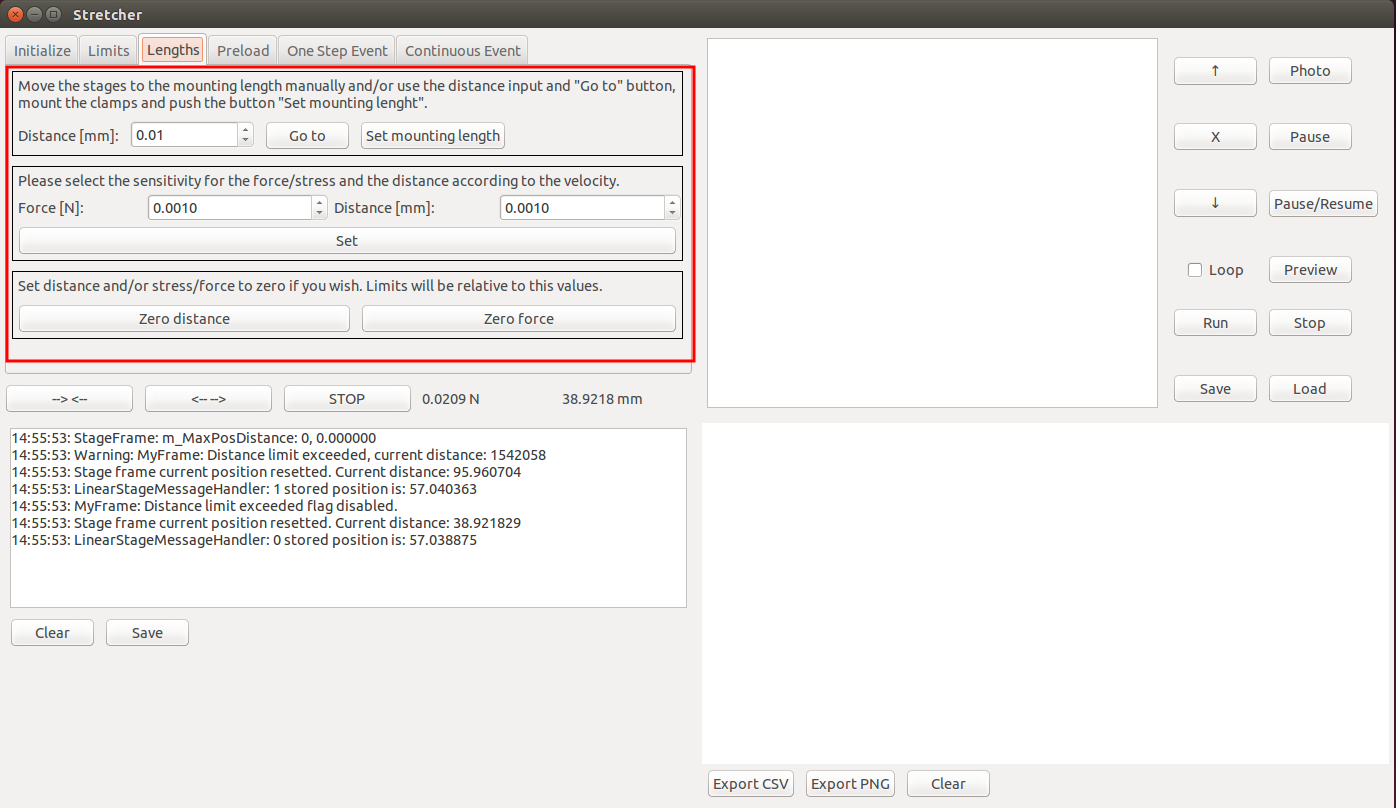
\includegraphics[width=1.0\textwidth]{images/Lengths}
	\caption{Lengths tab}
	\label{fig:lengths}
\end{figure}

It it is desired, the stress/force and the distance values can be zeroed by pushing the button ``Zero force'' respective ``Zero distance''.

\section{Homing of the stages}
If the stretcher software crashed, the stages were moved without the stretcher software or the stages aren't on the same position, the stages should be homed. In this case choose ``YES'' in the start-up dialog and then ``Cancel'' in the distance dialog. After that click on ``Home stages'' in the menu ``Advanced''. The homing dialog should appear with a warning message. Make sure, that nothing is mounted and nothing can break, if the stages go to their home position. If everything is clear, the button ``OK'' can be pushed which starts the homing of the two stages. In the next step, click on ``Start up dialog'' in the menu ``Advanced''. Now proceed as described in the section ``Normal start'' \ref{sec:normalstart}.

\begin{figure}[!ht]
	\centering
		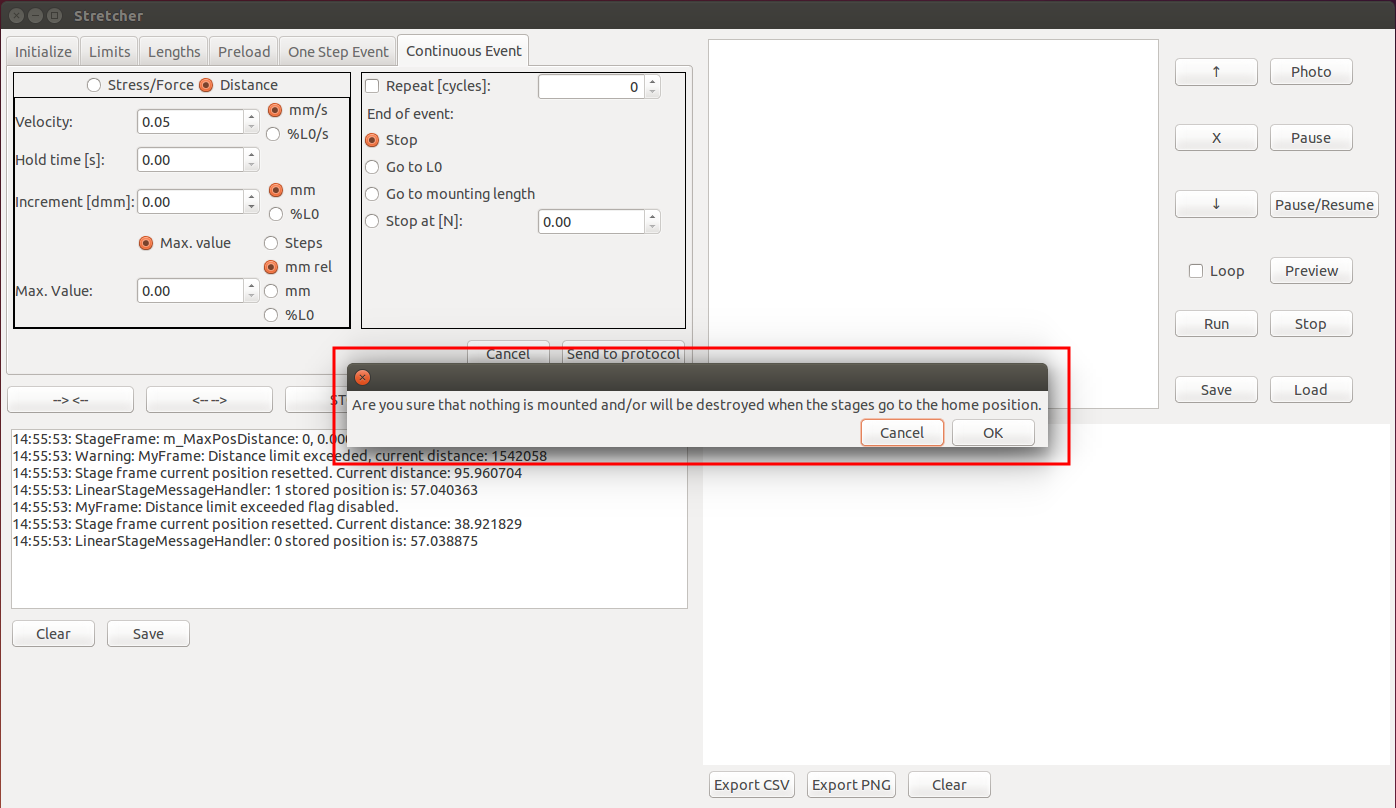
\includegraphics[width=1.0\textwidth]{images/HomeStages}
	\caption{Homing dialog}
	\label{fig:homeing}
\end{figure}
